\documentclass[border=2pt,tikz]{standalone}
\usepackage{tikz}
\usepackage{amsmath}
\usepackage{amssymb}
\usetikzlibrary{calc}

\def\centerarc[#1](#2)(#3:#4:#5) % Syntax: [draw options] (center) (initial angle:final angle:radius)
    { \draw[#1] ($(#2)+(#3:#5)$) arc (#3:#4:#5) node [right] {$\boldsymbol{\omega}$}; }

\begin{document}

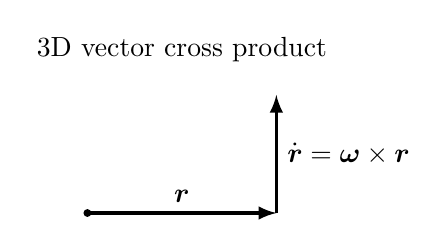
\begin{tikzpicture}[scale=3]

\node[above] at (0.4, 0.6) {3D vector cross product};

\def\r{0.20}

%\draw[draw=black] (-1,-1) rectangle (1,1);
%\draw (0,0) circle (\r);
\centerarc[very thick,->,>=latex](0,0)(45:315:\r)
\filldraw[black] (0.0,0.0)  circle (0.4pt);

\draw [very thick, ->,>=latex] (0,0) -- node [above] {$\boldsymbol{r}$} (0.8, 0.0) ;
\draw [very thick, ->,>=latex] (0.8, 0.0) -- node [right] {$\dot{\boldsymbol{r}}=\boldsymbol{\omega} \times \boldsymbol{r}$} (0.8, 0.5) ;

\end{tikzpicture}

\end{document}

